
%% bare_conf.tex
%% V1.4b
%% 2015/08/26
%% by Michael Shell
%% See:
%% http://www.michaelshell.org/
%% for current contact information.
%%
%% This is a skeleton file demonstrating the use of IEEEtran.cls
%% (requires IEEEtran.cls version 1.8b or later) with an IEEE
%% conference paper.
%%
%% Support sites:
%% http://www.michaelshell.org/tex/ieeetran/
%% http://www.ctan.org/pkg/ieeetran
%% and
%% http://www.ieee.org/

%%*************************************************************************
%% Legal Notice:
%% This code is offered as-is without any warranty either expressed or
%% implied; without even the implied warranty of MERCHANTABILITY or
%% FITNESS FOR A PARTICULAR PURPOSE! 
%% User assumes all risk.
%% In no event shall the IEEE or any contributor to this code be liable for
%% any damages or losses, including, but not limited to, incidental,
%% consequential, or any other damages, resulting from the use or misuse
%% of any information contained here.
%%
%% All comments are the opinions of their respective authors and are not
%% necessarily endorsed by the IEEE.
%%
%% This work is distributed under the LaTeX Project Public License (LPPL)
%% ( http://www.latex-project.org/ ) version 1.3, and may be freely used,
%% distributed and modified. A copy of the LPPL, version 1.3, is included
%% in the base LaTeX documentation of all distributions of LaTeX released
%% 2003/12/01 or later.
%% Retain all contribution notices and credits.
%% ** Modified files should be clearly indicated as such, including  **
%% ** renaming them and changing author support contact information. **
%%*************************************************************************


% *** Authors should verify (and, if needed, correct) their LaTeX system  ***
% *** with the testflow diagnostic prior to trusting their LaTeX platform ***
% *** with production work. The IEEE's font choices and paper sizes can   ***
% *** trigger bugs that do not appear when using other class files.       ***                          ***
% The testflow support page is at:
% http://www.michaelshell.org/tex/testflow/



\documentclass[conference]{IEEEtran}
% Some Computer Society conferences also require the compsoc mode option,
% but others use the standard conference format.
%
% If IEEEtran.cls has not been installed into the LaTeX system files,
% manually specify the path to it like:
% \documentclass[conference]{../sty/IEEEtran}


\usepackage[utf8]{inputenc}
\usepackage{graphicx}
\usepackage{hyperref}

% Some very useful LaTeX packages include:
% (uncomment the ones you want to load)


% *** MISC UTILITY PACKAGES ***
%
%\usepackage{ifpdf}
% Heiko Oberdiek's ifpdf.sty is very useful if you need conditional
% compilation based on whether the output is pdf or dvi.
% usage:
% \ifpdf
%   % pdf code
% \else
%   % dvi code
% \fi
% The latest version of ifpdf.sty can be obtained from:
% http://www.ctan.org/pkg/ifpdf
% Also, note that IEEEtran.cls V1.7 and later provides a builtin
% \ifCLASSINFOpdf conditional that works the same way.
% When switching from latex to pdflatex and vice-versa, the compiler may
% have to be run twice to clear warning/error messages.






% *** CITATION PACKAGES ***
%
%\usepackage{cite}
% cite.sty was written by Donald Arseneau
% V1.6 and later of IEEEtran pre-defines the format of the cite.sty package
% \cite{} output to follow that of the IEEE. Loading the cite package will
% result in citation numbers being automatically sorted and properly
% "compressed/ranged". e.g., [1], [9], [2], [7], [5], [6] without using
% cite.sty will become [1], [2], [5]--[7], [9] using cite.sty. cite.sty's
% \cite will automatically add leading space, if needed. Use cite.sty's
% noadjust option (cite.sty V3.8 and later) if you want to turn this off
% such as if a citation ever needs to be enclosed in parenthesis.
% cite.sty is already installed on most LaTeX systems. Be sure and use
% version 5.0 (2009-03-20) and later if using hyperref.sty.
% The latest version can be obtained at:
% http://www.ctan.org/pkg/cite
% The documentation is contained in the cite.sty file itself.






% *** GRAPHICS RELATED PACKAGES ***
%
\ifCLASSINFOpdf
  % \usepackage[pdftex]{graphicx}
  % declare the path(s) where your graphic files are
  % \graphicspath{{../pdf/}{../jpeg/}}
  % and their extensions so you won't have to specify these with
  % every instance of \includegraphics
  % \DeclareGraphicsExtensions{.pdf,.jpeg,.png}
\else
  % or other class option (dvipsone, dvipdf, if not using dvips). graphicx
  % will default to the driver specified in the system graphics.cfg if no
  % driver is specified.
  % \usepackage[dvips]{graphicx}
  % declare the path(s) where your graphic files are
  % \graphicspath{{../eps/}}
  % and their extensions so you won't have to specify these with
  % every instance of \includegraphics
  % \DeclareGraphicsExtensions{.eps}
\fi
% graphicx was written by David Carlisle and Sebastian Rahtz. It is
% required if you want graphics, photos, etc. graphicx.sty is already
% installed on most LaTeX systems. The latest version and documentation
% can be obtained at: 
% http://www.ctan.org/pkg/graphicx
% Another good source of documentation is "Using Imported Graphics in
% LaTeX2e" by Keith Reckdahl which can be found at:
% http://www.ctan.org/pkg/epslatex
%
% latex, and pdflatex in dvi mode, support graphics in encapsulated
% postscript (.eps) format. pdflatex in pdf mode supports graphics
% in .pdf, .jpeg, .png and .mps (metapost) formats. Users should ensure
% that all non-photo figures use a vector format (.eps, .pdf, .mps) and
% not a bitmapped formats (.jpeg, .png). The IEEE frowns on bitmapped formats
% which can result in "jaggedy"/blurry rendering of lines and letters as
% well as large increases in file sizes.
%
% You can find documentation about the pdfTeX application at:
% http://www.tug.org/applications/pdftex





% *** MATH PACKAGES ***
%
%\usepackage{amsmath}
% A popular package from the American Mathematical Society that provides
% many useful and powerful commands for dealing with mathematics.
%
% Note that the amsmath package sets \interdisplaylinepenalty to 10000
% thus preventing page breaks from occurring within multiline equations. Use:
%\interdisplaylinepenalty=2500
% after loading amsmath to restore such page breaks as IEEEtran.cls normally
% does. amsmath.sty is already installed on most LaTeX systems. The latest
% version and documentation can be obtained at:
% http://www.ctan.org/pkg/amsmath





% *** SPECIALIZED LIST PACKAGES ***
%
%\usepackage{algorithmic}
% algorithmic.sty was written by Peter Williams and Rogerio Brito.
% This package provides an algorithmic environment fo describing algorithms.
% You can use the algorithmic environment in-text or within a figure
% environment to provide for a floating algorithm. Do NOT use the algorithm
% floating environment provided by algorithm.sty (by the same authors) or
% algorithm2e.sty (by Christophe Fiorio) as the IEEE does not use dedicated
% algorithm float types and packages that provide these will not provide
% correct IEEE style captions. The latest version and documentation of
% algorithmic.sty can be obtained at:
% http://www.ctan.org/pkg/algorithms
% Also of interest may be the (relatively newer and more customizable)
% algorithmicx.sty package by Szasz Janos:
% http://www.ctan.org/pkg/algorithmicx




% *** ALIGNMENT PACKAGES ***
%
%\usepackage{array}
% Frank Mittelbach's and David Carlisle's array.sty patches and improves
% the standard LaTeX2e array and tabular environments to provide better
% appearance and additional user controls. As the default LaTeX2e table
% generation code is lacking to the point of almost being broken with
% respect to the quality of the end results, all users are strongly
% advised to use an enhanced (at the very least that provided by array.sty)
% set of table tools. array.sty is already installed on most systems. The
% latest version and documentation can be obtained at:
% http://www.ctan.org/pkg/array


% IEEEtran contains the IEEEeqnarray family of commands that can be used to
% generate multiline equations as well as matrices, tables, etc., of high
% quality.




% *** SUBFIGURE PACKAGES ***
%\ifCLASSOPTIONcompsoc
%  \usepackage[caption=false,font=normalsize,labelfont=sf,textfont=sf]{subfig}
%\else
%  \usepackage[caption=false,font=footnotesize]{subfig}
%\fi
% subfig.sty, written by Steven Douglas Cochran, is the modern replacement
% for subfigure.sty, the latter of which is no longer maintained and is
% incompatible with some LaTeX packages including fixltx2e. However,
% subfig.sty requires and automatically loads Axel Sommerfeldt's caption.sty
% which will override IEEEtran.cls' handling of captions and this will result
% in non-IEEE style figure/table captions. To prevent this problem, be sure
% and invoke subfig.sty's "caption=false" package option (available since
% subfig.sty version 1.3, 2005/06/28) as this is will preserve IEEEtran.cls
% handling of captions.
% Note that the Computer Society format requires a larger sans serif font
% than the serif footnote size font used in traditional IEEE formatting
% and thus the need to invoke different subfig.sty package options depending
% on whether compsoc mode has been enabled.
%
% The latest version and documentation of subfig.sty can be obtained at:
% http://www.ctan.org/pkg/subfig




% *** FLOAT PACKAGES ***
%
%\usepackage{fixltx2e}
% fixltx2e, the successor to the earlier fix2col.sty, was written by
% Frank Mittelbach and David Carlisle. This package corrects a few problems
% in the LaTeX2e kernel, the most notable of which is that in current
% LaTeX2e releases, the ordering of single and double column floats is not
% guaranteed to be preserved. Thus, an unpatched LaTeX2e can allow a
% single column figure to be placed prior to an earlier double column
% figure.
% Be aware that LaTeX2e kernels dated 2015 and later have fixltx2e.sty's
% corrections already built into the system in which case a warning will
% be issued if an attempt is made to load fixltx2e.sty as it is no longer
% needed.
% The latest version and documentation can be found at:
% http://www.ctan.org/pkg/fixltx2e


%\usepackage{stfloats}
% stfloats.sty was written by Sigitas Tolusis. This package gives LaTeX2e
% the ability to do double column floats at the bottom of the page as well
% as the top. (e.g., "\begin{figure*}[!b]" is not normally possible in
% LaTeX2e). It also provides a command:
%\fnbelowfloat
% to enable the placement of footnotes below bottom floats (the standard
% LaTeX2e kernel puts them above bottom floats). This is an invasive package
% which rewrites many portions of the LaTeX2e float routines. It may not work
% with other packages that modify the LaTeX2e float routines. The latest
% version and documentation can be obtained at:
% http://www.ctan.org/pkg/stfloats
% Do not use the stfloats baselinefloat ability as the IEEE does not allow
% \baselineskip to stretch. Authors submitting work to the IEEE should note
% that the IEEE rarely uses double column equations and that authors should try
% to avoid such use. Do not be tempted to use the cuted.sty or midfloat.sty
% packages (also by Sigitas Tolusis) as the IEEE does not format its papers in
% such ways.
% Do not attempt to use stfloats with fixltx2e as they are incompatible.
% Instead, use Morten Hogholm'a dblfloatfix which combines the features
% of both fixltx2e and stfloats:
%
% \usepackage{dblfloatfix}
% The latest version can be found at:
% http://www.ctan.org/pkg/dblfloatfix




% *** PDF, URL AND HYPERLINK PACKAGES ***
%
%\usepackage{url}
% url.sty was written by Donald Arseneau. It provides better support for
% handling and breaking URLs. url.sty is already installed on most LaTeX
% systems. The latest version and documentation can be obtained at:
% http://www.ctan.org/pkg/url
% Basically, \url{my_url_here}.




% *** Do not adjust lengths that control margins, column widths, etc. ***
% *** Do not use packages that alter fonts (such as pslatex).         ***
% There should be no need to do such things with IEEEtran.cls V1.6 and later.
% (Unless specifically asked to do so by the journal or conference you plan
% to submit to, of course. )


% correct bad hyphenation here
\hyphenation{op-tical net-works semi-conduc-tor}


\begin{document}
%
% paper title
% Titles are generally capitalized except for words such as a, an, and, as,
% at, but, by, for, in, nor, of, on, or, the, to and up, which are usually
% not capitalized unless they are the first or last word of the title.
% Linebreaks \\ can be used within to get better formatting as desired.
% Do not put math or special symbols in the title.
\title{Método de Segmentación Probabilistico de Cerebro\\ Utilizando Imagenes MRI}


% author names and affiliations
% use a multiple column layout for up to three different
% affiliations
\author{\IEEEauthorblockN{Cristóbal Donoso}
\IEEEauthorblockA{Dpto. Ciencias de la Computación\\Facultad de Ingeniería\\
Universidad de Concepción, CHILE\\
Email: cridonoso@udec.cl}
\and
\IEEEauthorblockN{Pamela Guevara y Claudio Roman}
\IEEEauthorblockA{Dpto. Ing. Biomedica\\Facultad de Ingeniería\\
Universidad de Concepción, CHILE\\
Email: pguevara@udec.cl, clauroman@udec.cl}
}

% conference papers do not typically use \thanks and this command
% is locked out in conference mode. If really needed, such as for
% the acknowledgment of grants, issue a \IEEEoverridecommandlockouts
% after \documentclass

% for over three affiliations, or if they all won't fit within the width
% of the page, use this alternative format:
% 
%\author{\IEEEauthorblockN{Michael Shell\IEEEauthorrefmark{1},
%Homer Simpson\IEEEauthorrefmark{2},
%James Kirk\IEEEauthorrefmark{3}, 
%Montgomery Scott\IEEEauthorrefmark{3} and
%Eldon Tyrell\IEEEauthorrefmark{4}}
%\IEEEauthorblockA{\IEEEauthorrefmark{1}School of Electrical and Computer Engineering\\
%Georgia Institute of Technology,
%Atlanta, Georgia 30332--0250\\ Email: see http://www.michaelshell.org/contact.html}
%\IEEEauthorblockA{\IEEEauthorrefmark{2}Twentieth Century Fox, Springfield, USA\\
%Email: homer@thesimpsons.com}
%\IEEEauthorblockA{\IEEEauthorrefmark{3}Starfleet Academy, San Francisco, California 96678-2391\\
%Telephone: (800) 555--1212, Fax: (888) 555--1212}
%\IEEEauthorblockA{\IEEEauthorrefmark{4}Tyrell Inc., 123 Replicant Street, Los Angeles, California 90210--4321}}




% use for special paper notices
%\IEEEspecialpapernotice{(Invited Paper)}




% make the title area
\maketitle

% As a general rule, do not put math, special symbols or citations
% in the abstract

\begin{abstract}
El cerebro es una estructura anatómicamente difícil de segmentar. Para abordar este problema es necesario aplicar técnicas computacionales cuyo desempeño optimice el proceso. En el siguiente trabajo se presenta la aplicación de un método probabilístico que utiliza modelos ocultos de Markov para modelar espacialmente cada tejido en el cebrero. \\
\end{abstract}
\begin{center}
https://github.com/cridonoso/tumor\_detection
\end{center}
% no keywords




% For peer review papers, you can put extra information on the cover
% page as needed:
% \ifCLASSOPTIONpeerreview
% \begin{center} \bfseries EDICS Category: 3-BBND \end{center}
% \fi
%
% For peerreview papers, this IEEEtran command inserts a page break and
% creates the second title. It will be ignored for other modes.
\IEEEpeerreviewmaketitle



\section{Introduction}
La segmentación en imágenes es un problema difícil de resolver. Esto debido a la complejidad en la representación y estructura de los datos; por ejemplo dependencias espaciales. En  particular, el cerebro es una estructura difícil de tratar debido a su anatomía.\\\\Las imágenes de resonancia magnética (MRI) permiten capturar tridimensionalmente distintos tejidos del cerebro, sin embargo, segmentar cada parte puede ser bastante lento y depende del paciente - ya que el cerebro no es rígido y su forma varía considerablemente persona a persona. 
\begin{figure}[h]
\begin{center}
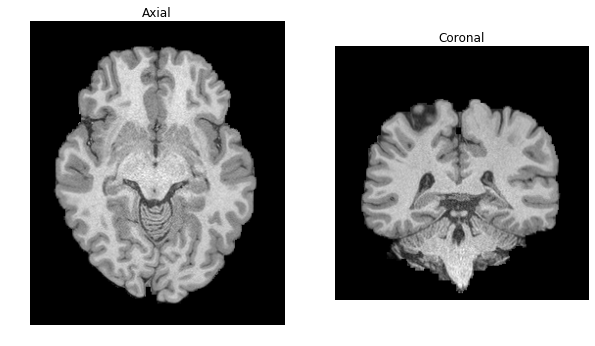
\includegraphics[scale=0.4]{img/brain_real.png} 
\end{center}
\caption{Corte coronal y axial desde una imagen nifti cerebro completo}
\end{figure}
En este contexto, se hace necesario desarrollar técnicas computacionales que realicen segmentación de tejidos cerebrales con el objetivo de optimizar el desempeño. Una buena alternativa, es abordar este problema desde un punto de vista probabilístico. A continuación, se revisará un método probabilístico de segmentación espacial. Luego se presentarán los principales resultados del método sobre un conjunto de pacientes. 

\section{Descripción del Algoritmo}
En este trabajo se aplicó un modelo estadístico de segmentación de cerebro. El modelo utiliza un ensamblaje de técnicas lo cual aumenta la efectividad de los objetivos esperados. En general, cuando queremos abordar el problema de segmentación nos encontramos con dos características fundamentales:
\begin{enumerate}
\item Basado en ciertas métricas, nuestro modelo debe agrupar términos semejantes asignándole una etiqueta de clase.
\item La distribución de un punto debe considerar información espacial. Por ejemplo, si estamos identificando tejidos en una imagen; dos tejidos pueden tener una intensidad semejante, sin embargo no forman parte de un mismo cuerpo.
\end{enumerate}
En relación a estos dos puntos (Zhang et.al 2001) propone un modelo llamado Hiden Markov Random Field (HMRF), el cual desarrolla segmentación mediante un proceso estocástico haciendo uso de variables aleatorias ocultas. El algoritmo encuentra el grado de pertenencia de un pixel a una etiqueta mediante el cálculo del posterior. La distribución posterior consiste en el producto entre la verosimilitud (desde los datos) y el prior (conocimiento a priori del fenómeno)
\begin{equation}
\mathrm{posterior} \propto \mathrm{prior} \times \mathrm{likelihood}
\end{equation}
\begin{equation}
p^t(l | y_i) = \frac{g^t(y_i;\phi_l)p^t(l|x_{N_i}) }{p(x)}
\end{equation}
En específico estamos estimando la probabilidad de un píxel dada una etiqueta.  El algoritmo, estocásticamente, mejora los parámetros del modelo en búsqueda de un óptimo que entregue una buena generalización del caso de estudio (segmentación).
Este procedimiento se realiza por medio de modelos ocultos de Markov, el cual entrega secuencias de observaciones (Random fields).
\begin{equation}
p(y|x) = \prod_{i\in S} P(y_i | x_i)
\end{equation}
Las secuencias establecen relaciones de condicionalidad entre variables aleatorias.\\\\La información espacial entre píxeles está considerada en la teoría de Random Fields. En particular, un pixel $x_i$ se relaciona con otro $x_j$ ssi este último pertenece a la vecindad de $x_i$. Una vecindad  de $x_i$ lo conforman todos los pixeles $x_{s-\{i\}}$, donde S es el conjunto de vecinos. Luego podemos determinar las probabilidades condicionales $P(x_i | x_{N_i})$ donde $N_i$ = $S-{i}$. Este sistema puede ser multidimensional (en nuestro experimento utilizamos imágenes .nifti tridimensionales).
\section{Resultados}
Para los experimentos se utilizaron muestras de 5 pacientes. De cada paciente teniamos la mascara corresponiente a la referencia de materia blanca y gris. Por cada mascara generada calculamos el coeficiente de Sorensen-Dice
\begin{equation}
s = \frac{2|X \cap Y|}{|X| + |Y|}
\end{equation}
donde X e Y son la mascara generada por el modelo y la de referencia respectivamente. A continuación se muestran los resultados calculando el coeficiente para el cerebro completo y cada hemisferio; $p_i$ corresponde al paciente $i-$ésimo.

\begin{table}
\caption{Resultados Coeficiente deSorensen-Dice }
\begin{center}
\begin{tabular}{|c|c|c|c|c|c|}
\hline 
Paciente & $p_1$ & $p_2$ & $p_3$ & $p_4$ & $p_5$ \\ 
\hline 
\hline
Completo &  0.9325 & 0.9357 & 0.9260 & 0.9343 & 0.9312 \\ 
\hline 
Izquierdo & 0.9585 & 0.9596 & 0.9493 & 0.9601 & 0.9563 \\ 
\hline 
Derecho & 0.9571 & 0.9642 & 0.9517 & 0.9595 & 0.9574 \\ 
\hline 
\end{tabular}\\
\end{center} 
{\footnotesize Tabla 1: Tabla de resultados para el coeficiente de Sorensen-Dice entre las mascara del modelo (una por cada paciente) y la de referencia (una por cada paciente)}
\end{table}

Para buscar la mejor mascara, iteramos sobre todas las slides generadas por nuestro modelo probabilistico. A su vez, comparabamos la similitud de pixeles correspondientes con la mascara. El grafico de la figura 1 muestra la cantidad de puntos coincidentes entre la slide del modelo y la de referencia. De esta manera buscamos la mejor mascara (veáse la figure 2)
\begin{figure}
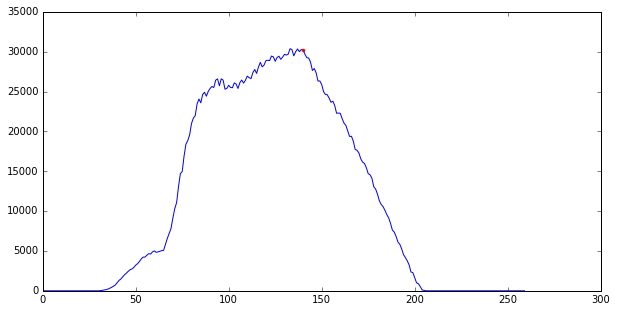
\includegraphics[scale=0.4]{img/best_mask.png} 
\caption{Grafico que muestra los puntos en comun para cada par de slides (una para el modelo y otra de referencia)}
\end{figure}
\begin{figure}
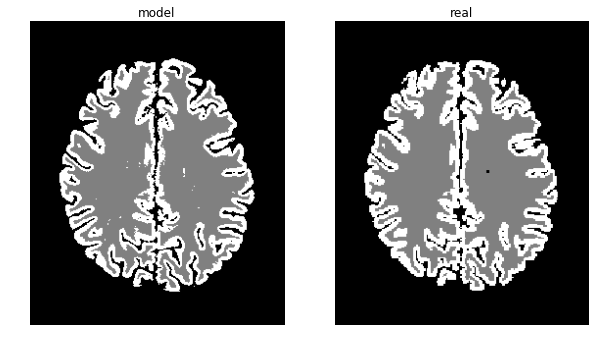
\includegraphics[scale=0.4]{img/brain_mask.png}\\
\caption{[izquierda] imagen de la mascara generada por el modelo [derecha] imagen de referencia. Ambas mascaras muestran materia blanca y gris}
\end{figure}
\section{Conclusión}
Los resultados calculados se acercan al óptimo (mascara de referencia). Es claro que el modelo logra ajustarse a los datos entregando una distribución capaz de segmentar la imagen. No obstante, el tiempo que toma este algoritmo no es menor debido a la cantidad de operaciones que realiza. Para ello, es posible intentar con métodos más inteligentes que aprendan a segmentar desde la misma imagen sin necesidad de calcular estadísticos (por ej. una red neuronal convolucional).\\\\\\\\\

\begin{thebibliography}{1}
\bibitem{IEEEhowto:kopka}
Zhang, Y., Brady, M., \& Smith, S. (2001). Segmentation of brain MR images through a hidden Markov random field model and the expectation-maximization algorithm. IEEE transactions on medical imaging, 20(1), 45-57.
\bibitem{IEEEhowto:kopka}
Avants, B. B., Tustison, N. J., Wu, J., Cook, P. A., \& Gee, J. C. (2011). An open source multivariate framework for n-tissue segmentation with evaluation on public data. Neuroinformatics, 9(4), 381-400.


\end{thebibliography}




% that's all folks
\end{document}


